\chapter{Theory of Dark Matter}
\label{chapter:DM}
% add what does the different method excludes in the Dark Matter summary plot


\epigraph{\textit{One does not become enlightened by imagining figures of light, but by making the darkness conscious.}}{--Carl Jung}

%TODO: 1. Evidence Large scale structure of the universe
% 	   2. SUSY and long lived particle model and signature
%      3. 
Dark Matter is one of the most solid pieces of evidence for Beyond-the-Standard-Model physics. In 1933, Fritz Zwicky first conceptualized the existence of a dunkle Materie (``Dark Matter") holding the galaxies to the cluster center and thus preventing them from flying apart~\cite{Zwicky}. The proposition was later concurred by different findings by Horace W. Babcock~\cite{Babcock} and Jan Oort~\cite{oort}, among many others. 

It is estimated that Dark Matter makes up about 25\% of the existing matter-energy composition of the universe, about 5 times more than ordinary matter(See Figure~\ref{fig:planck}). It plays a major role in astrophysical object formation and the evolution of the universe. 

Dark Matter is known for interacting gravitationally and at most weakly (though recent evidence has shown weak scale interaction to be unlikely~\cite{DM2016}). It does not interact electromagnetically or strongly. As various cosmological surveys and astrophysics analyses has revealed more Dark Matter properties, it does not match that of any SM particle. Its creation, composition and interaction mechanisms are not yet understood.

Different theoretical candidates have since been proposed for Dark Matter, which includes primordial blackholes, massive compact halo objects(MACHOs), and weakly interactng massive particles(WIMPs) to name a few. A popular theory proposes that Dark Matter is made up of particles, just like ordinary matter. Under this hypothesis, Dark Matter would be a different kind of particle(s) that is governed by physics in the ``dark sector" not yet included in the Standard Model.

    Many experiments use different ways to search for Dark Matter particles. Experiments range from satellite telescopes that hunts for photon excess from possible Dark Matter interactions, to Earth target experiments that attempt to capture Dark Matter that travels through the planet. Experiments that seek to further understand the nature of Dark Matter also include the Large Hadron Collider: the machine features many experiments that seeks to produce Dark Matter through extreme high energy intensity collisions of subatomic particles. This thesis will feature three different analyses that seek to find Dark Matter with this method. 

    In this chapter, evidence for Dark Matter is reviewed in Section~\ref{section:evidence}, Dark Matter and the current properties that restrict its nature will be covered in Section~\ref{section:properties}, and Section~\ref{section:candidates} reviews possible Dark Matter candidates. An overview of search methods for Dark Matter as a particle is covered in Section~\ref{section:searches}; highlights of the theoretical modeling approach used by the LHC of Dark Matter are discussed in Section~\ref{section:models}. Lastly, LHC Dark Matter search signatures are discussed in Section~\ref{section:signatures}.

\section{Evidence}
\label{section:evidence}

The evidence for dark matter include galactic rotational curvees, gravitational lensing and cosmic microwave background.

\subsection{Galactic Rotational Curve}
The first proposition of Dark Matter was in the 1930s by Fritz Zwicky based on observation of the Coma cluster. It was later confirmed by further systematic galaxy rotational curve studies by Vera Rubin, Kent Ford~\cite{Rubin} and Ken Freeman~\cite{freeman}.  

    Most of the studies can be interpreted following Zwicky's original argument: galactic clusters and galaxies are treated as stable systems of discrete particles at astrophysical scale. They are therefore governed by the Virial Theorem:

\begin{equation}
     \langle T \rangle = -\frac{1}{2} \sum_{k=1}^{N} \langle F_{k} \cdot r_{k} \rangle
    \label{eq:virial}
\end{equation}

Here T represents kinetic energy, F is the force that holds the particles in the system together, and r is the distance between the particles, and N is the total number of particles in the system. 

    The Virial Theorem states that there is a direct correlation between the kinetic energy and potential energy in a particle system. In other words, there is a correlation between the velocity of the object (through kinetic energy) and the mass (through gravitational force) of the system. 
    The correlation is as the following:
    
     $$ v(r) \varpropto \frac{M(r)}{\sqrt{r}}, $$ 
     where v is the velocity, r is the distance from the center of the system and M(r) is the mass of the galaxy enclosed by a sphere with a radius of r. 

     In these observational studies, the striking finding was that the velocity distribution for many of these clusters and galaxies do not follow the prediction from the Virial Theorem: the velocity curves of the galaxies do not follow the expected $\frac{1}/\frac{\sqrt{r}}$ distribution, instead, they are close to constant to r, especailly in the outer rings. Figure~\ref{M33_figure} shows the difference between the theoretical prediction and the observation. 

     Since the galactic rotational curves studies are performed on the luminous objects that can be observed through light, which means invisible matter could just not be accounted for. One proposed solution to the problem is to add a halo of non-luminous Dark Matter to these galaxies. The additional mass would then make the galactic rotational curves match the Virial Theorem prediction. As the result is found across many galaxies studied, galactical rotational curves are seen as major evidence for the existence of Dark Matter. 

\begin{figure}[!htb]
    \begin{center}
        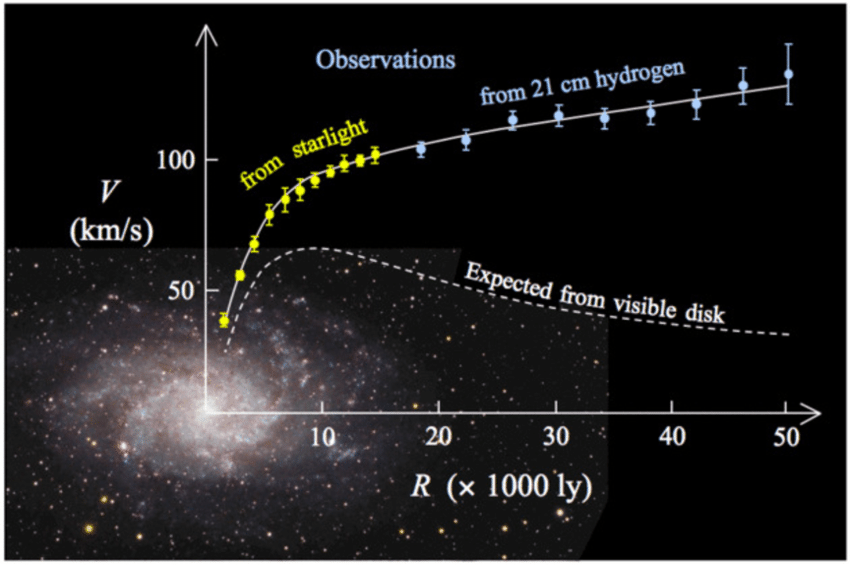
\includegraphics[width=0.75\textwidth]{figures/chapter_DM/M33-rotation-curve}
        \caption{
            The galactic rotational curve of M33. The expected rotational curve is shown in the dotted line. Experimental data is shown in yellow and in blue~\cite{M33}.
        }
        \label{fig:M33_figure}
    \end{center}
\end{figure}

\subsection{Gravitational Lensing}
General relativity verdicts that massive objects bend space-time around them. The details are captured elegantly in the Einstein's Equation~\ref{eq:Einstein}. 

\begin{equation}
	R_{\mu \nu} - {1 \over 2}R \, g_{\mu \nu} + \Lambda g_{\mu \nu}= {8 \pi G \over c^4} T_{\mu \nu}, 
    \label{eq:Einstein}
\end{equation}

In this equation, $R_{\mu \nu}$ is the Ricci curvature tensor, R is the scalar curvature. Together, they form the Einstein tensor. $g_{\mu \nu}$ is the metric tensor, and $T_{\mu \nu}$ is the stress-energy tensor. This equation states that the curvature of space-time is directly related to the mass and energy in that space. 	
	
	Consequently, light rays that travel through the curved space-time around the massive object are therefore ``bent". The effect is analogous to the effect of angled lenses bending light rays due to a velocity difference across different media, and is called ``gravitational lensing". 

    There are different forms of this lensing effect: ``Strong lensing" happens when bending of light result in either multiple images. Or, as a light ring or light arcs observed around massive centers of galaxy clusters and galaxies; ``Weak lensing" usually involves weaker spatial distortion effects over many objects in a region; micro-lensing is when the effect is only an apparent change in the brightness of the source.

    Dark Matter's existence is evident from gravitational lensing studies. An example of strong lensing that demonstrates existence of Dark Matter is shown in Figure~\ref{fig:BulletCluster_figure} in the bullet cluster collision of 1E 0657-56~\cite{BulletCluster}. The image is produced from the combination of gravitational lensing and x-ray telescope imaging. The red part of the diagram denotes ordinary matter and the blue part represents Dark Matter. In the cluster collision, ordinary matter
    bend light around them and became luminous from the collision, captured by x-ray imaging; The blue part shows a part of the cluster that did not interact luminously and was only inferred through gravitational lensing. This is a strong evidence for the existence of non-luminous matter in the clusters. The observation also constrains the self-interaction of Dark Matter.

    Weak lensing results of galaxies distribution over a large area has provided further evidence and constrained the for density and distribution of Dark Matter in the universe~\cite{wittman2000detection}.


\begin{figure}[!htb]
    \begin{center}
        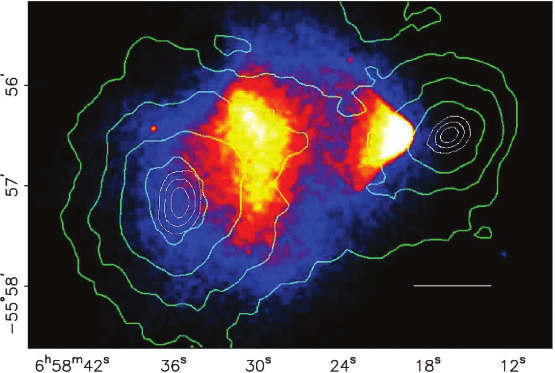
\includegraphics[width=0.75\textwidth]{figures/chapter_DM/BulletCluster}
        \caption{
			Bullet cluster (1E 0657-56) showing two colliding galaxy clusters, the part in red came from x-ray image by Chandra, highlighting normal matter distribution; the part in blue came from gravitational lensing~\cite{BulletCluster}.
        }
        \label{fig:BulletCluster_figure}
    \end{center}
\end{figure}

\subsection{Cosmic Microwave Background}
\label{sec:CMB}
In the beginning of the universe, ordinary matter and Dark Matter existed in a hot plasma soup with frequent interaction between charged particles and photons. As the universe continued to expand, during a period called ``recombination", the expansion of the universe had cooled the plasma soup enough that charged particles began to form neutral atoms. Photons do not scatter on the neutral atoms, and thus propagate to the other end of the universe. Due to red shifting, they form a microwave
background of the universe that can still be observed today. This is the Comic Microwave Background (CMB). The CMB is very uniform, but there are still small temperature variations. Figure~\ref{fig:CMB} display the CMB along with its temperature variations~\cite{fixsen2009temperature}. The variations came from primordial acoustic oscillation that came from the interaction of Dark Matter and ordinary matter with photons in the original plasma. It can be decomposed into an angular power spectrum.

Due to the different interaction rate between Dark Matter and ordinary matter with photons and each other, different Dark Matter and ordinary matter make-up of the universe would result in different angular spectroscopy shapes, the angular spectroscopy data can be fitted to find the composition of the universe. Figure~\ref{fig:CMBfigure} shows a fitted angular spectroscopy. From the result, it was found that Dark Matter is not only an essential part of the universe, its composition is approximately 5 times as large as ordinary matter. 

\begin{figure}[!htb]
    \begin{center}
        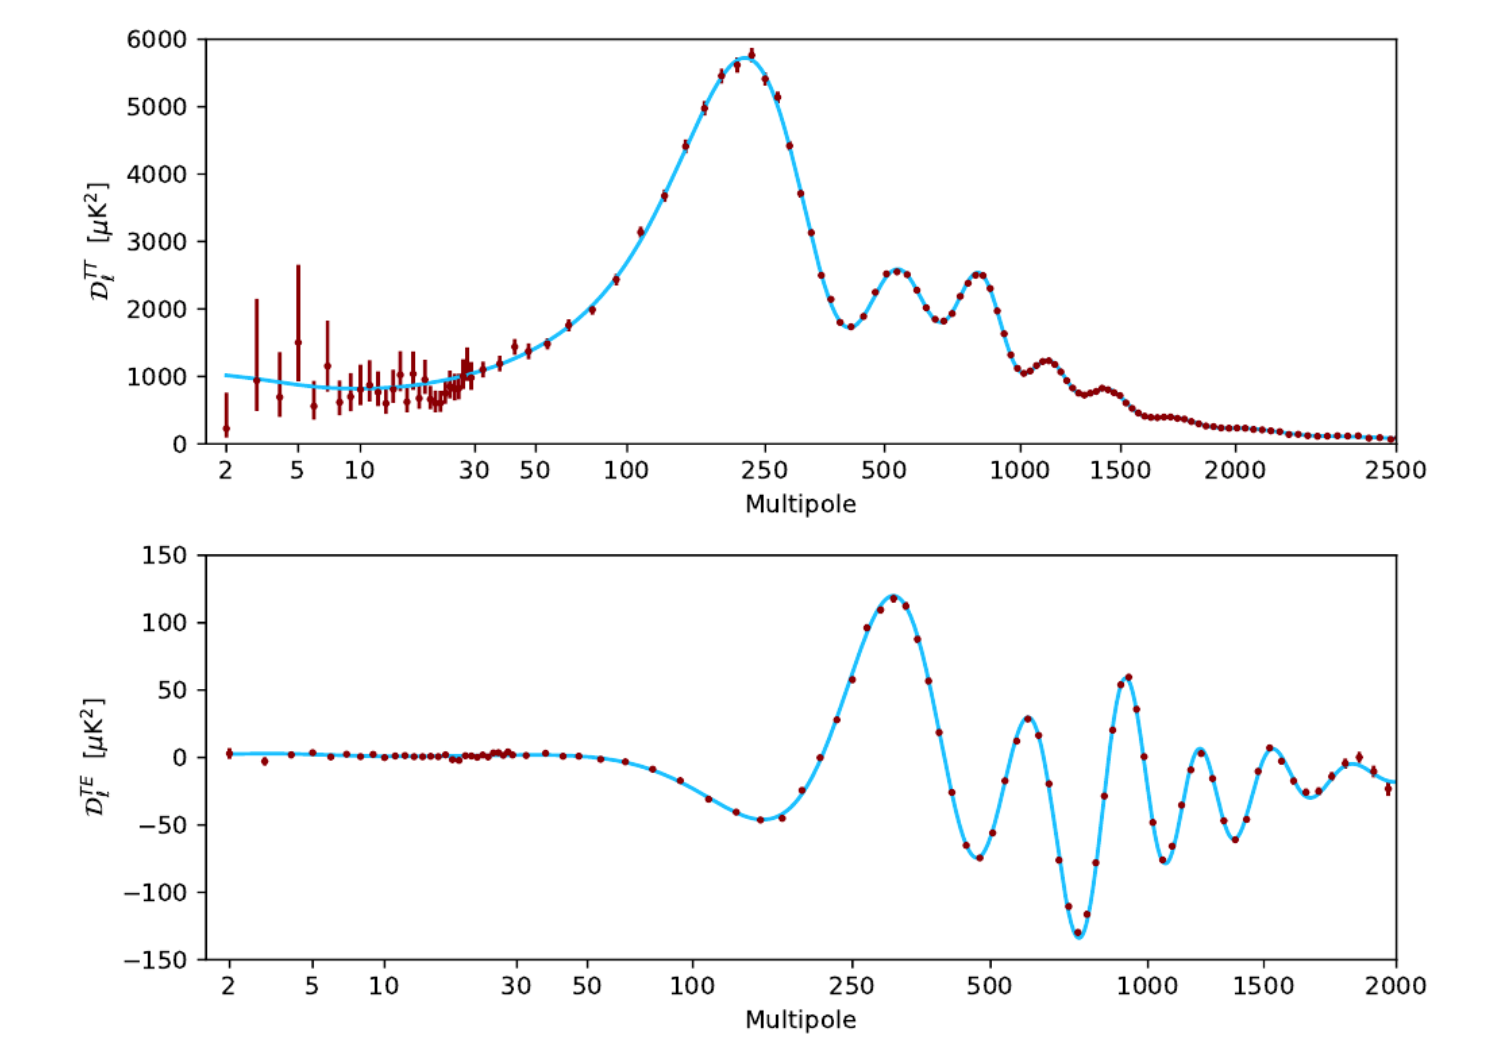
\includegraphics[width=0.75\textwidth]{figures/chapter_DM/CMB-angular-power-spectrum}
        \caption{
			The Cosmic Microwave Background power spectrum measured by Planck~\cite{CMB}.
        }
        \label{fig:CMBfigure}
    \end{center}
\end{figure}

\section{Properties of Dark Matter}
\label{section:properties}
While Dark Matter itself has never been directly observed, many studies in the cosmological, astrophysical and particle scales have constrained many of its properties. In this section throughout this thesis, the following properties of Dark Matter will be discussed and justified.

\subsection{Dark}
Measurement of Dark Matter got its name from its little to no interaction with light, compared to ordinary matter. Collision of the bullet cluster has also greatly constrained its interaction with itself\  
It is taken that it will not interact with collider detectors. Its interaction with ordinary matter would be rare in the energy scale of the LHC. 

\subsection{Long Life Time}
As Dark Matter is seen today in evidence across different scales (see Section~\ref{section:evidence}). It is assumed to have a long life time since the age of the universe. Many theoretical models of Dark Matter require a $Z_{2}$ symmetry, such as the R parity of supersymmetry. This prevents Dark Matter particles from decaying into lighter SM objects. In most experimental searches today, it is be treated as something that does not decay further into other detectable SM
particles~\cite{boveia2018dark}.

\subsection{Interacts Gravitationally}
Current evidence (see section~\ref{section:evidence}) suggests that Dark Matter is massive, and thus interacts gravitationally. However, there is no consensus on the mass on the individual constituents of Dark Matter. 

\subsection{Cold}
Current theoretical candidates of Dark Matter can be split into two camps: ``cold" Dark Matter and ``hot" Dark Matter. The former group suggests that Dark Matter is made of objects massive enough, therefore the velocity would be non-relativistic; the latter group suggest the opposite view. There is evidence in support of both hypotheses. The Dark Matter candidates being searched for in the rest of the thesis will be assumed to be cold, as this property allows for its search in the LHC under certain signature. The justification for Dark Matter as a cold particle came analysis of galaxy formation and the process requires Dark Matter to be above a certain mass. 
% cold dark matter citation.

\subsection{Low Self Interaction}
Dark Matter is believed to have little to no self interaction. Mixed X-ray, optical and gravitational lensing studies on the merging galacy cluster 1E-657-65 has restricted its self interaction limit to below $\frac{\sigma}{m}= < 1.25 cm^{2} g^{-1}$ (68\% confidence)~\cite{randall2008constraints}. 
 
%\subsection{Single Particle}
%While there are many composite Dark Matter models being proposed these days, Dark Matter is still taken to be a single kind in most effective model/simplified model building for experimental searches. 

\section{Candidates}
\label{section:candidates}
There exist a wide range of candidates for what Dark Matter could be. Here, a few possible candidates for Dark Matter are outlined.

\subsection{Sterile Neutrino}
The SM does not predict that neutrinos have a mass, but this contradicts with experimental findings and is therefore a problem for the SM. By replacing right-handed neutrinos in the SM with gauge singlet fermions that have no interaction other than mixing with normal neutrinos. Sterile neutrino is formed by theoretical models. On tuning parameters such as its its interaction rate with normal neutrinos, mass and mixing angle, sterile neutrino can be a possible candidate for Dark
Matter, which can lead to a density of Dark Matter with stability consistent with the scale of the universe~\cite{dodelson1994sterile}. They are searched for in radiator experiments such as the Daya Bay~\cite{an2014search, wong2017search} and in scintillator experiments like DANSS~\cite{alekseev2018search}.

% Mass and range  mass keV scale, currently sterile neutrino mass is unknown and therefore can be either hot or cold
%Daya Bay Collaboration, F. P. An et al., “Search for a Light Sterile Neutrino at Daya Bay,” Phys. Rev. Lett. 113 (2014) 141802, arXiv:1407.7259 [hep-ex].
%1310.8642
\subsection{Axion}

Another existing problem in the SM is the strong CP problem, the problem is described in detail in Section~\ref{sec:strongcp}. One natural solution to the problem is to introduce an additional symmetry called the Peccei-Quinn symmetry~\cite{peccei1977cp}, which would lead to an mediator particle called the axion. 

The axion proposed is a Dark Matter candidate, as it shares many properties with the known profile of Dark Matter including an exceptionally long life time. Recent experimental finding from the XENON1T experiment shows anomalies that could be signs of axions~\cite{aprile2020excess}.
%ADMX mass mu eV
%https://arxiv.org/pdf/2104.01406.pdf
%Xenon Collaboration, E. Aprile et al,. "Excess Electronic Recoil Events in XENON1T", Phys. Rev. D 102, 072004 (2020), arXiv: 2006.09721


% Non-particle candidates
%\subsection{Modified Newtonian Gravity}
%\subsection{MACHOs}

\subsection{Weakly Interacting Massive Particle (WIMP)}
A very attractive candidate for Dark Matter is called the weakly interacting massive particle(WIMP). It appears naturally with many Beyond-the-Standard-Model theories that aim to solve other physics problems, including theories of supersymmetry with R-parity and some extra dimensional theory. 
In the study of Dark Matter in cosmology, it is frequently assumed to be a thermal relic. Thermal relic Dark Matter is in thermal equilibrium with ordinary matter in the early universe. In thermal equilibrium with ordinary matter, it gets produced and annihilated at the same rate. There comes a point in the universe called ``freezing out", where the expansion of the universe cools the particle bath and the temperature becomes lower than the energy required for Dark Matter to be produced given
Dark Matter mass. Dark Matter production from ordinary matter thus ceased. As the universe further expands, it becomes more difficult for Dark Matter to find each other annihilated and form ordinary matter. Dark Matter abundance is locked at this point and remain unchanged until today. Figure ~\ref{fig:WIMP_figure} shows a plot that demonstrates how thermal relics work. Using this model and the current measured abundance of Dark Matter in our current universe, the self annihilation cross section of Dark Matter is $ \langle \sigma \cdot v \rangle \simequal 3 \cdot 10^{26}cm^{3} s^{-1}$. This annihilation cross section scale matches many prediction made in supersymmetry theories. Many Beyond-the-Standard-Model theories, such as SUSY, the Universal Extra Dimension Model, and the little Higgs all predict a particle with known Dark Matter properties and self-interaction rate of the same scale. This is known as the WIMP miracle~\cite{Dev_2014}.

%\Figure WIMP miracle


\begin{figure}[!htb]
    \begin{center}
        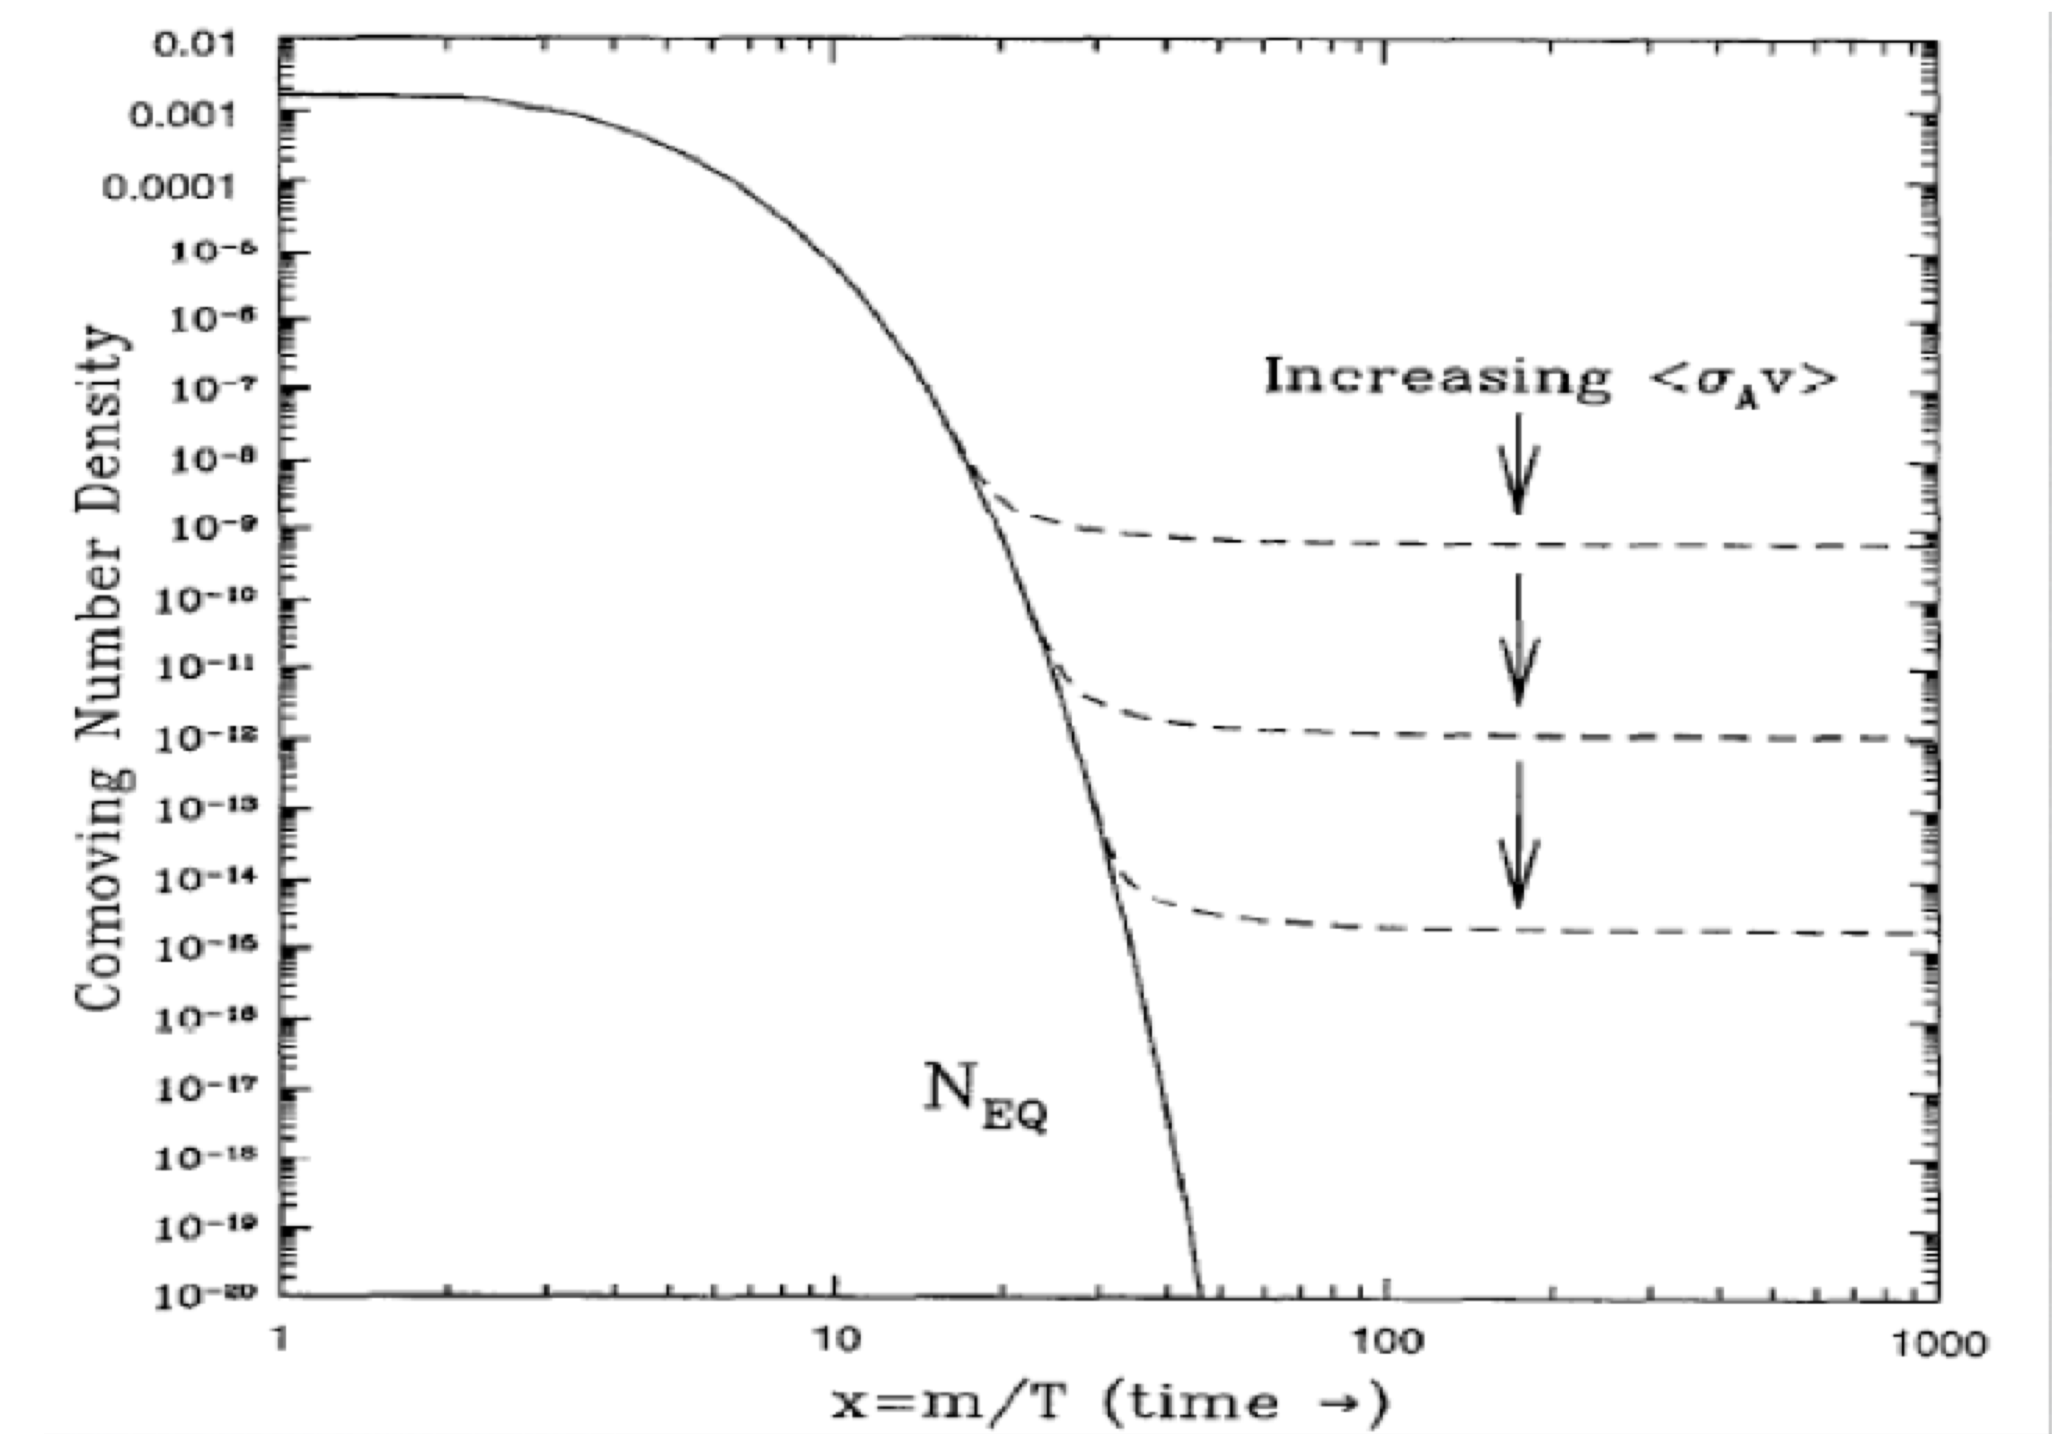
\includegraphics[width=0.75\textwidth]{figures/chapter_DM/WIMP}
        \caption{
            Solid line here shows the change in the densitiy of Dark Matter in an expanding unverse. In the early universe, the solid is horizontal, indicating the time when Dark Matter production and annihilation is equal. The line gradually fall with increase of time when production rate began to decrease with the universe expansion. Later as the universe further expands, the annihilation stops as well and Dark Matter gets freezes out to different density level with different assumed self interaction annihilation rates~\cite{WIMP}.
        }
        \label{fig:WIMP_figure}
    \end{center}
\end{figure}


 

%P.S. BHUPAL DEV, ANUPAM MAZUMDAR, & SALEH QUTUB, FRONT.IN PHYS. 2 (2014) 26
%https://indico.cern.ch/event/473000/contributions/1993414/attachments/1209863/1764345/tait-Aspen.pdf

%https://www.particlebites.com/?p=7004
%https://www.forbes.com/sites/startswithabang/2019/02/22/the-wimp-miracle-is-dead-as-dark-matter-experiments-come-up-empty-again/?sh=5ebc59f46dbc

\section{Experimental Search Overview}
\label{section:searches}

Traditionally the search for Dark Matter is split into different experimental categories sorted by the different detection methods from different Dark Matter/ordinary matter interactions. 

\begin{figure}[!htb]
    \begin{center}
        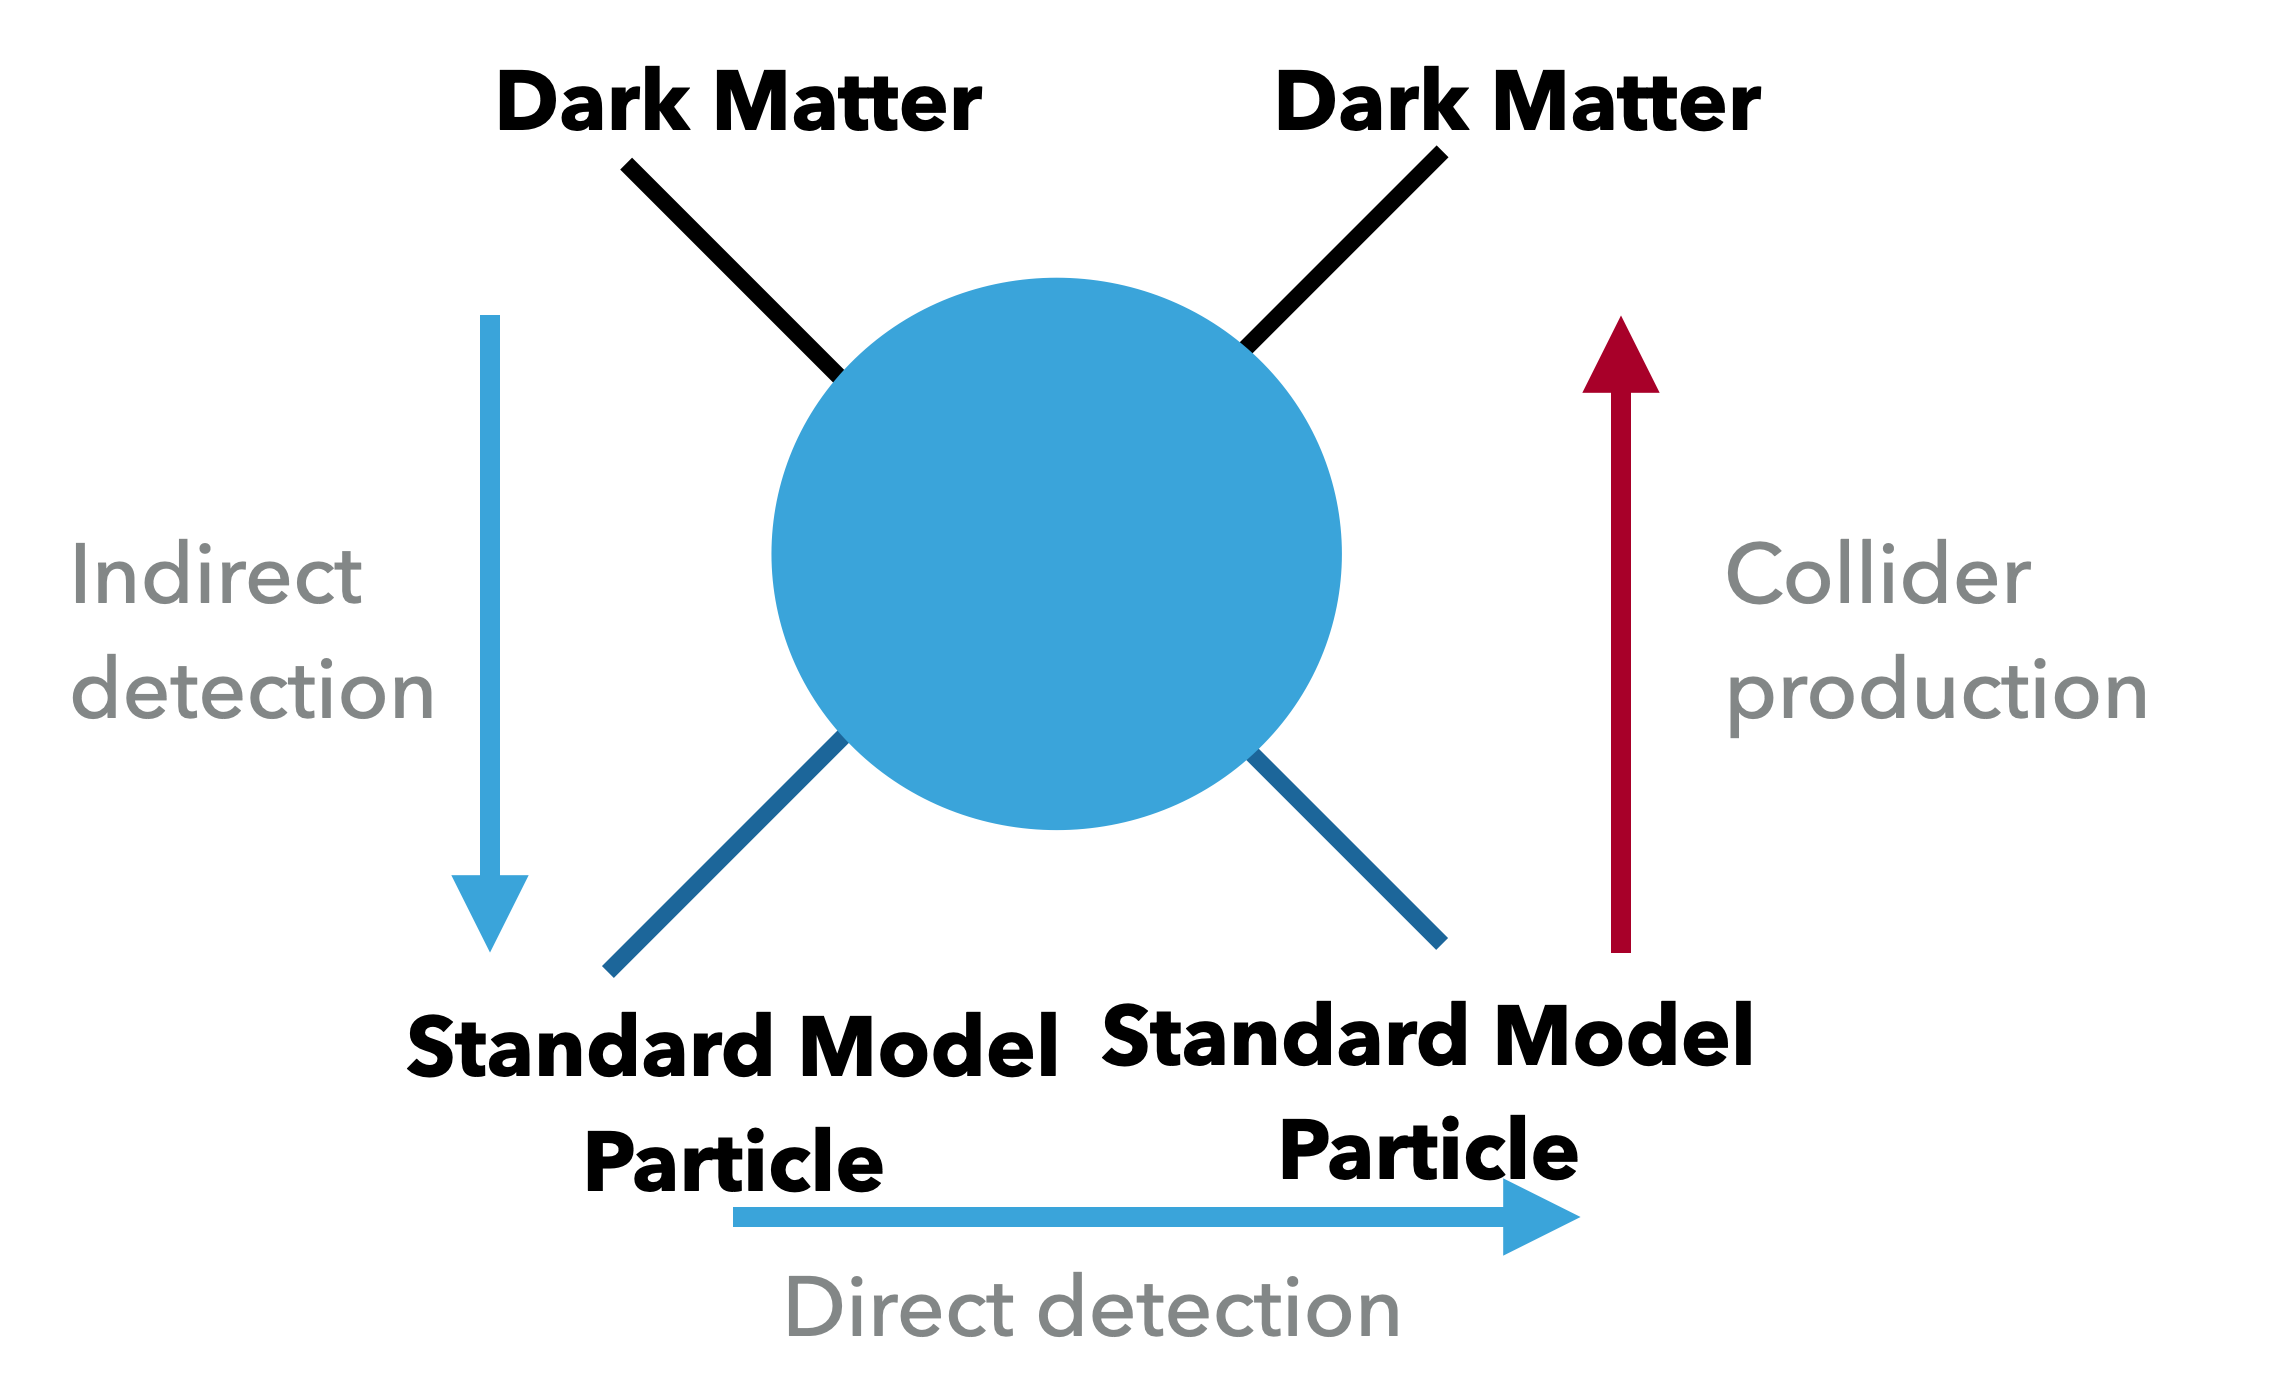
\includegraphics[width=0.75\textwidth]{figures/chapter_DM/Interaction}
        \caption{
			Schematic cartoon showing the different Dark Matter detection methods facilitated by different interactions thus signatures. 
        }
        \label{fig:interaction}
    \end{center}
\end{figure}

\subsection{Direct Detection}
Dark Matter is believed to travel across the universe through the earth. Assuming weak interaction between Dark Matter and SM nucleons, Dark Matter can be detected directly with different target objects. 

\begin{equation}
    R \propto N \rho \chi \langle \sigma_{\chi } \rangle
\end{equation}

Here, R is the interaction rate, N is the number of events $\rho$ is the density of the target object, $\chi$ is the interaction area for each event decay and $\sigma_{\chi}$ is the interaction cross section. 

There are many experiments that use different interaction material and target different Dark Matter masses. Notable experiments include LZ~\cite{mckinsey2016lz}, Xenon1T~\cite{aprile2020excess}, SuperCDMS~\cite{Agnese_2016}, CRESST~\cite{Angloher_2014} and DAMA~\cite{Bernabei_2008}. 

As more experiments had excluded much of the theory model phasespace, many of the experiments now face the challenge of the ``neutrino floor" in low mass Dark Matter searches, where the neutrino background in cosmic radiation begins to dominate signal regions. 

\subsection{Indirect Detection}
Indirect detection looks for SM annihilation products of Dark Matter. It looks for interaction in places where matter is dense enough to interact, usually in center of galaxies and stars. Experiments include FermiLAT~\cite{albert2017searching} and H.E.S.S.~\cite{aharonian2006hess}.

\subsection{Collider Production} 
In colliders, Dark Matter can be studied by being directly produced from SM particles. As this will be the method that the rest of the thesis is based on, 
the theoretical models as well as the experimental signatures of Dark Matter in the LHC will be discussed in detailed in Section~\ref{section:models} and Section~\ref{section:signatures}.

\section{Theoretical Models in LHC Searches}
\label{section:models}
While there exist a wide range of speculation on the identity of Dark Matter, LHC as a Dark Matter searching tool can only probe a unique set of Dark Matter candidates.

Different approaches are used to develop benchmark models when searching for Dark Matter at the LHC. The choice of model is a trade-off between simpicity, physics reinterpretability and experimental sensitivity. Sorting by an ascending degree of completeness, this section will review the different approaches and models of Dark Matter used at the LHC. Figure~\ref{fig:Model_figure} shows the theoretical models used in the LHC sorting from its level of completeness.

\begin{figure}[!htb]
    \begin{center}
        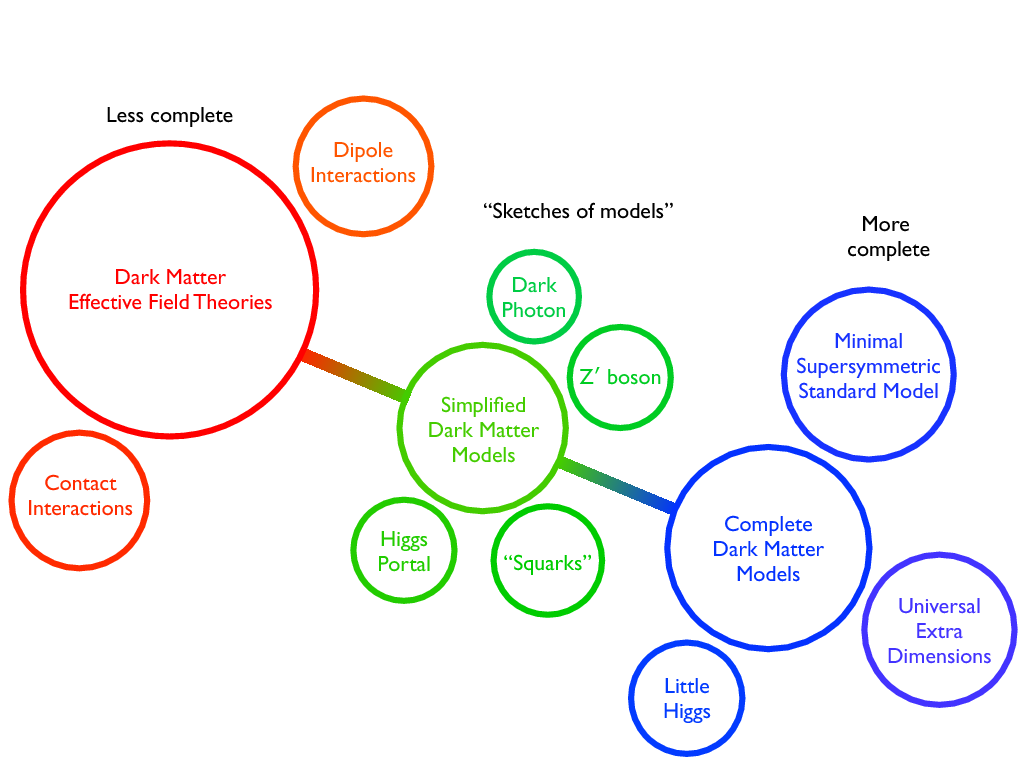
\includegraphics[width=0.75\textwidth]{figures/chapter_DM/Model}
        \caption{
			Colored Scheme showing Dark Matter modeling approach from more simplistic (left) to more complete models (right)~\cite{Abdallah:2024101}.
        }
        \label{fig:Model_figure}
    \end{center}
\end{figure}

\subsection{Simple Portal Models}
The simplest kind of models are simple extensions to the SM. In these models, Dark Matter is mediated either through the Higgs or the Z Boson. As the Z portal models are constrained by LEP and DD experiments (LUX, PandaX-II), Dark Matter that are mediated through a heavier version of Z boson (the $Z\prime$) and additional scalar are also searched for and are sometimes regarded as the simple portal models.

\subsection{Effective Field Theory}
\label{sec:EFT}
The effective field theory (EFT) approach condenses a wide range of complete models their simplified versions by focusing on what is experimentally accessible. High mass mediator particles in complete theories act as a contact operator. High energy correction and details are integrated out for ``effectiveness". All kinematically accessible observables are described by a Lorentz structure and a rate parameter. 

This approach allow for measured experimental values to be directly converted to theory parameters. A wide range of complete models can be probed with a few clear experimental model search. However, the model has a singularity and is not valid for when the interaction momentum transfer is close to that of the mediator mass. In the LHC, Monte Carlo(MC) event generation, which is the standard computer simulation of collision events that are used to aid studies, a truncation method is used to bound
the simulated Monte Carlo events below this singularity limit~\cite{Busoni_2014}.

\subsection{Simplified Model}
The singularity problem in EFT can be resolved with a simplified model approach. In simplified model, the contact interaction in EFT is turned into mediator particle s-channel/t-channel exchanges. With the price of an increased number of parameters, simplified models can provide the full mechanics of a particle interaction with the additional details. 

Simplified models of Dark Matter at the LHC do not break the global and gauge symmetries of SM, the Lagrangian terms are Lorentz invariant and predict at least a Dark Matter candidate that fullfills the properties requirements in the previous section. 

Some simplified Dark Matter model used in the LHC include the Two-Higgs Doublet Model (2HDM)~\cite{TwoHiggs2012}, where Higgs or a non-SM exotic Higgs could serve as a mediator to Dark Matter; as well as dark photon or kinetically mixed Z' Dark Matter models. 

Other than these, simplified model in supersymmetry such as the Phenomenological Minimal Supersymmetric SM (pMSSM)~\cite{pMSSM1996}, which reduces the over 100 parameters of the complete Minimal Supersymmetric SM to 19 parameters, predicts a natural Dark Matter candidate, neutralino. 

In addition, other gauge or gravity mediated SUSY theory predicts the gravitino as a Dark Matter candidate. 
% pMSSM Assumes no sources of CP violation Beyond-the-Standard-Model and no flavor-changing neutral currents, and retains uni- versal couplings and masses for first- and second-generation superpartners. %CatDog Antonio DM summary paper.  

\subsection{Less-simplified models}
Simplified models are able to capture common features in many Dark Matter models, but it neglects features from other models. As the LHC work towards expanding its search signatures, the less-simiplified models are becoming more popular. These include non-minimally flavor violating models, coannihilation models that include two or more kinds of Dark Matter particles, as well as multiple Higgs models where the additional exotic Higgs serves as a mediator between SM particles and Dark Matter. The
signatures for these models are captured in Figure~\ref{fig:Less-Simplified}.

\begin{figure}[!htb]
    \begin{center}
        \includegraphics[width=0.75\textwidth]{figures/chapter_DM/Less-Simplified}
        \caption{
            Figure here shows the signature for the less-simplified models which include the non-minimally flavor violating monotop signature, a possible signature from the coannihilation model, as well as an exotic Higgs signature~\cite{DMSearchatCollider2018}.
        }
        \label{fig:Less-Simplified}
    \end{center}
\end{figure}

A detailed list of models used at the LHC by both CMS and ATLAS can be found in ~\cite{Abercrombie_2020}.
%\subsection{Long-Lived Particle Models}

%\subsection{Long-Lived Particle Models}


\subsection{The LHC Dark Matter Benchmark}
\label{sec:LHCDM}
The Dark Matter benchmark from the LHC uses the EFT approach (described in Section~\ref{sec:EFT}). It encompasses a wide range of Dark Matter models with its signature. 

In the Dark Matter benchmark of the LHC, the SM is extented by an additional U(1) symmetry: it is assumed that Dark Matter along with some Stanard Model particles are all charged under this. A new gauge boson can thereby facilitate interaction between the SM and Dark Matter field. 

The Dark Matter mediator can either be an axial vector or a vector. The corresponding lagrangians are:

\begin{equation}
\mathcal{L}_{vector}= g_{q} \sum_{q=u,d,s,c,b,t} Z'_{\mu}\bar{q}\gamma^{\mu}q + g_{\chi}Z'_{\mu}\bar{\chi}\gamma^{\mu}\chi
\end{equation}

\begin{equation}
\mathcal{L}_{axial vector}= g_{q} \sum_{q=u,d,s,c,b,t} Z'_{\mu}\bar{q}\gamma^{\mu}\gamma^{5}q + g_{\chi}Z'_{\mu}\bar{\chi}\gamma^{\mu}\gamma^{5}\chi
\end{equation}

Here, $\mathcal{L}_{vector}$ and $\mathcal{L}_{axial vector}$ represent the Lagrangian for the Dark Matter interaction, $Z\prime$ represents the field for the Dark Matter mediator; $g_{\chi}$ is the interaction strength, $\gamma$ are the dirac matrices and q are the different quark fields\footnote{u, d, s, c, b, t represents up, down, strange, charm, bottom and top}.

Under this calculation the minimal parameters of the model is reduced to ${g_{q}, g_{\chi}, m_{\chi}, M_{med}}$. 
Similar argument can be made for lepton decays where the quark decays are replaced by leptons. 

%On ATLAS, these models are generated in the event generator with NLO+PS accuracy with the POWHEG generator, the product goes through parton showering at PYTHIA8 with detector simulation from GEANT4. 

\section{Experimental Signature in the LHC}
\label{section:signatures}
This section review some common signatures of dark matter that are being searched for at the LHC.

\subsection{Mono-X signature}
\label{sec:monoX}
    This describes the type of Dark Matter search where an invisible Dark Matter particle is produced directly at the LHC and is ``observed" in the detector as missing transverse momentum.
    Dark Matter is known to interact only very weakly with normal matter, and thus is assumed to not leave a trace in the LHC detector. When events are produced through proton-proton collision along the z-axis in the LHC, the momentum of all objects along the transverse plane to the z-axis is always zero. Therefore, when an event has missing transverse momentum recoiling against another visible object, the signature could possibly be Dark Matter.
This class of analysis is named by the SM object that Dark Matter recoils against. Mono-jet, mono-Higgs, mono-Z are a few analyses done this way. 

\subsection{Di-object Signature}
    Dark Matter can also be searched for without the production of the Dark Matter particle. The simplified models that predicts Dark Matter in the mono-X analyses predicts effective mediator particle between SM particle with Dark Matter. These effective mediator particles can be directly searched for through via decay back into SM objects. As the process is distinct from any known SM particle processes, an excess of events beyond the known Standard Model prediction could be indicative of Dark Matter in the LHC. These di-object search include dijet, dilepton, diphoton searches. In recent years, new techniques such as the trigger-level-analysis and channels that have an additional initial state radiation objects are being pioneered. These result in a search phasespace much greater than the traditional program and greatly extended the of the richness of the LHC serach program.

\subsection{Supersymmetry Invisible Particles}
There are a few natural candidate in SUSY that could match the profile of Dark Matter being searched for, they show up in detector signatures as missing transverse momentum. Many searches in SUSY that aims for missing tranverse momentum has more complicated decay chains with multiple particles compared to the signature presented in Section~\ref{sec:monoX}
So far, no searches on SUSY has found anything statistically significant, but the increased data size has led to new exploration in the electrowino phasespace.

\subsection{Search for Long-Lived Particles}
The LHC is also looking for a new set of decay channels as well as missing transverse momentum dark matter signatures through Long-Lived particles searches. These signatures are predicted by extensions to SUSY models~\cite{LongLived2020}. Long-Lived particles can decay inside the tracking detector, or calorimeters and sometimes even outside of the main detectors. The observation of these particles are somtimes challenging due to the required dedicated triggers and specified reconstruction algorithms. 

%\subsection{Supersymmetric Signature}	

%\subsection{Long-Lived Particle Signature}

%\subsection{Long-Lived Particle Signature}


%The Signature used for this analysis 
%\subsection{}
